\documentclass[12pt]{article}
\usepackage{enumerate}
\usepackage{notes}
\usepackage{oxford}

\begin{document}
\title{Oxford A1 - Differential Equations \footnotetext{\url{https://courses.maths.ox.ac.uk/node/5372}}}
\author{Dan Davison}
\maketitle

\begin{comment}
\section{Sheet 1}

\subsection*{} % 1
\begin{mdframed}
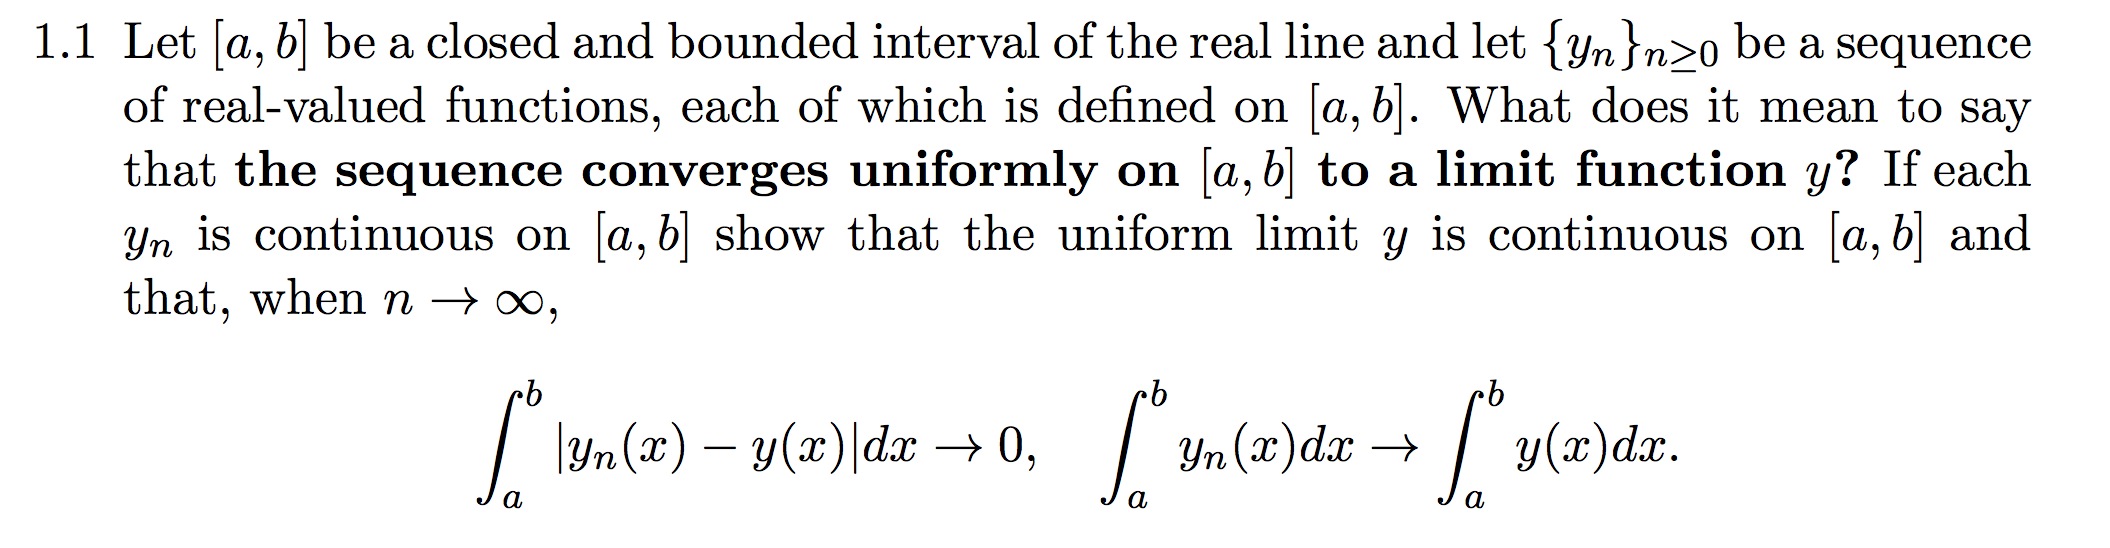
\includegraphics[width=450pt]{img/differential-equations-a1-1-1-a.png}
\end{mdframed}

\subsubsection*{(a) Definition of uniform convergence}
The sequence of functions $\{y_n\}_{n\geq 0}$ \textbf{converges uniformly on
  $[a, b]$ to $y$} if and only if for all $\epsilon > 0$ there exists an
$m \in \N$ such that for all $n > m$ and for all $x \in [a,b]$,
$|y_n(x) - y(x)| < \epsilon$.

\subsubsection*{(b) Show that the limit function is continuous}

The claim is that if each $y_n$ is continuous on $[a,b]$ then $y$ is
continuous on $[a,b]$. We are told that
\begin{enumerate}
\item $\{y_n\}_{n \geq 0}$ converges uniformly to $y$, and
\item each $y_n$ is continuous on $[a,b]$.
\end{enumerate}
~\\
\textbf{Informal illustration of proof:}\\
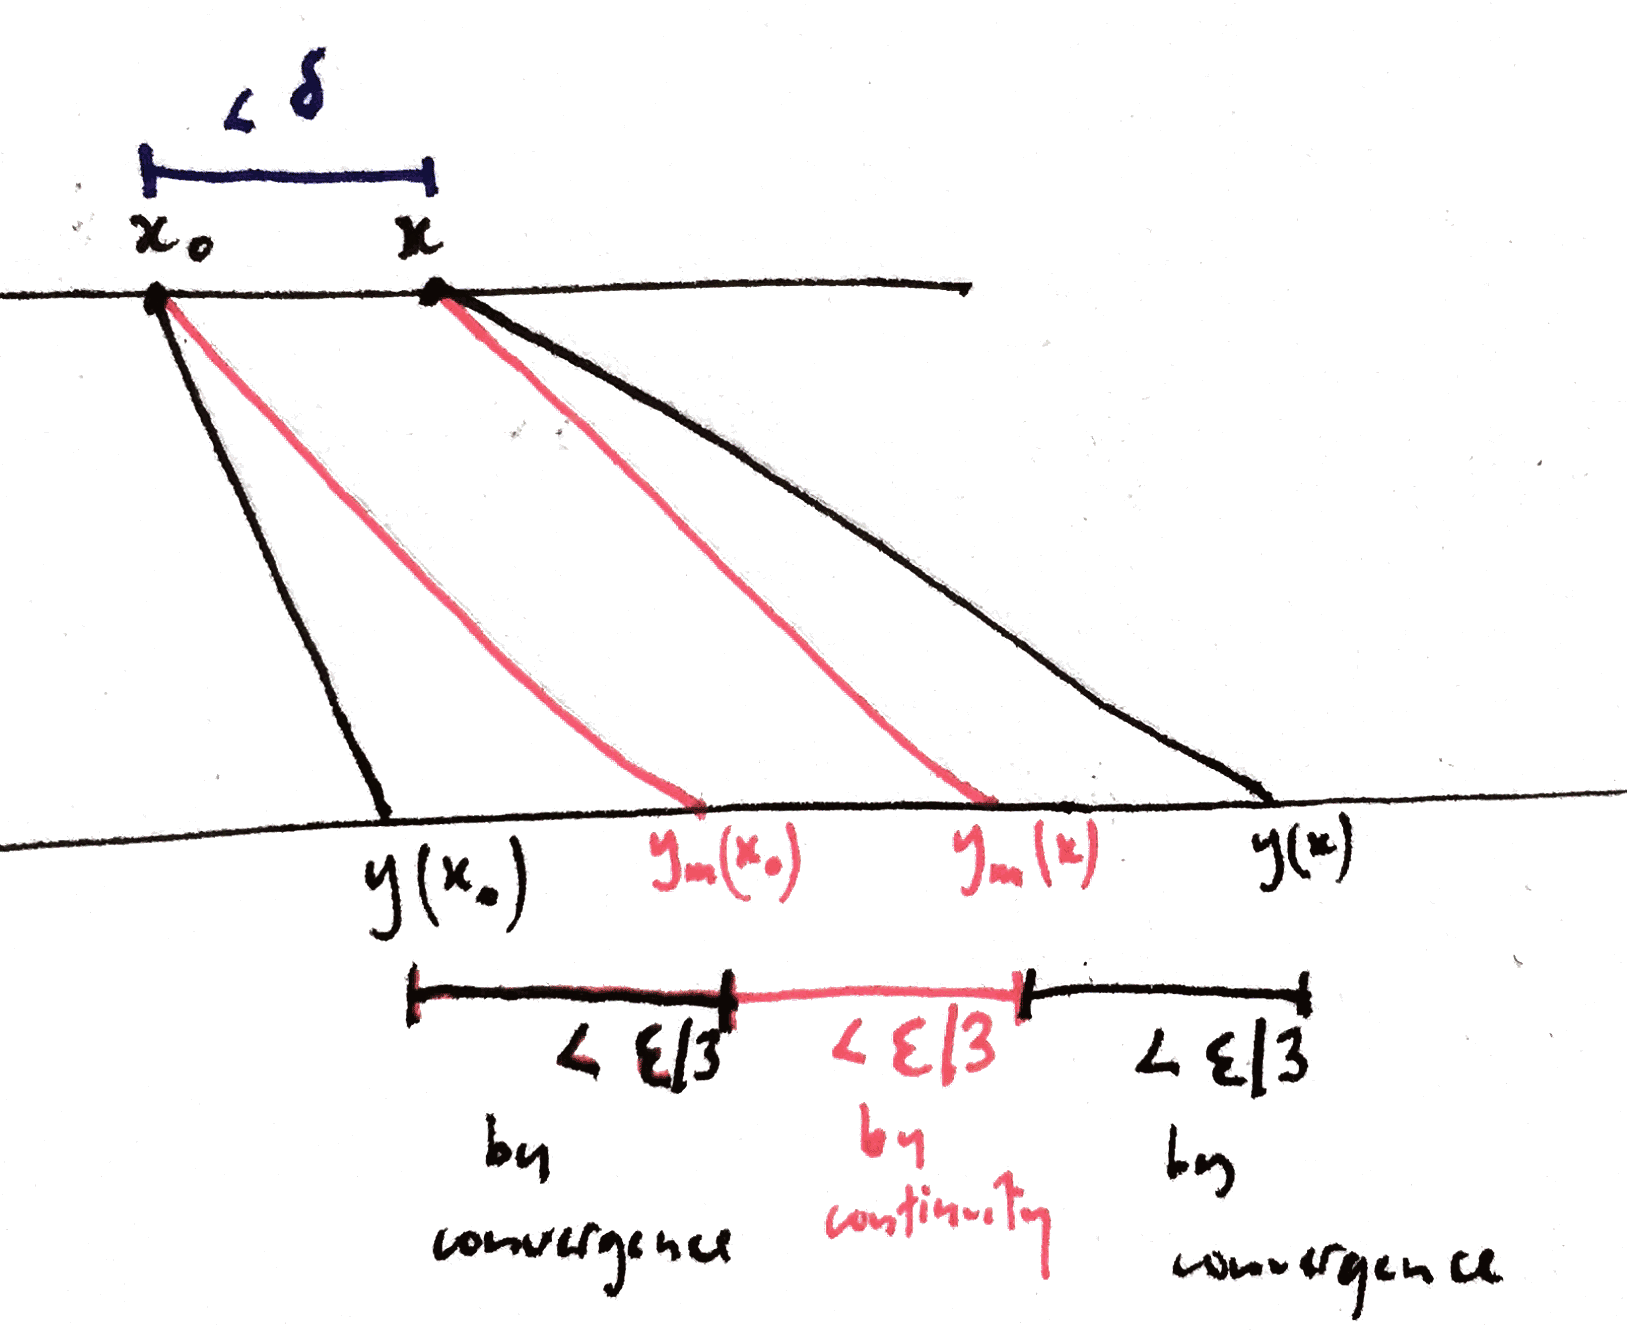
\includegraphics[width=200pt]{img/differential-equations-a1-1-1-a-diagram.png}\\

% We need to show that for every $\epsilon > 0$, for every $x_0 \in [a, b]$,
% there exists a $\delta > 0$ such that
% $|x - x_0| < \delta \implies |y(x) - y(x_0)| < \epsilon$.

Fix arbitrary $\epsilon > 0$ and $x_0 \in [a,b]$.

Let $m \in \N$ be such that $|y_m(x_0) - y(x_0)| < \epsilon/3$. Such an $m$
exists because the $\{y_n\}$ converge uniformly to $y$.

Let $\delta$ be such that
$|x - x_0| < \delta \implies |y_m(x) - y_m(x_0)| < \epsilon/3$. Such a
$\delta$ exists because $y_m$ is continuous on $[a,b]$.

Fix an arbitrary $x$ such that $|x - x_0| < \delta$.

Now we have the following:
\begin{enumerate}
\item $|y(x_0) - y_m(x_0)| < \epsilon/3$ ~~~~ by convergence of the $\{y_n\}$
\item $|y_m(x_0) - y_m(x)| < \epsilon/3$ ~~~ by continuity of $y_m$
\item $|y_m(x) - y(x)| < \epsilon/3$    ~~~~~~ by convergence of the $\{y_n\}$
\end{enumerate}
Therefore $|y(x_0) - y(x)| < \epsilon$, proving continuity of $y$ on $[a,b]$. \qed

\blue{(Approximate time taken for reading and producing an answer: 4hrs)}

\subsubsection*{(c) Show limit of definite integral I}

Let $I_n = \int_a^b |y_n(x) - y(x)| \dx$.

The claim is that $\lim_{n \to \infty} I_n = 0$.

In other words
$\forall \epsilon > 0: \exists~ m \in \N: \forall~ n > m: |I_n - 0| <
\epsilon$.

Fix an $\epsilon > 0$.

Since the $\{y_n\}$ converge uniformly to $y$, there exists an $m \in \N$
such that for all $n > m$ and for all $x \in [a,b]$
\begin{align*}
  |y_n(x) - y(x)| < \epsilon/(b-a).
\end{align*}

Therefore $\int_a^b |y_n(x) - y(x)| \dx < \epsilon$ for all $n > m$, as required. \qed

\subsubsection*{(d) Show limit of definite integral II}

The claim is that $\lim_{n \to \infty} \int_a^b y_n(x) \dx = \int_a^b y(x) \dx$.

In other words:
$\forall \epsilon > 0: \exists~ m \in \N: \forall~ n > m:$
\begin{align*}
  \Big|\(\int_a^b y_n(x) \dx\) - \(\int_a^b y(x) \dx\)\Big| < \epsilon.
\end{align*}

This is equivalent to:
$\forall \epsilon > 0: \exists~ m \in \N: \forall~ n > m:$
\begin{align*}
  A_1 := \Big|\int_a^b \(y_n(x) - y(x)\) \dx\Big| < \epsilon.
\end{align*}

From part (c) above, we know that:
$\forall \epsilon > 0: \exists~ m \in \N: \forall~ n > m:$
\begin{align*}
  A_2 := \int_a^b |y_n(x) - y(x)| \dx < \epsilon.
\end{align*}

Now\footnote{This is related to the triangle inequality. I should prove it
  properly.} if the sign of $y_n(x) - y(x)$ is constant for all $x \in [a,b]$
(i.e. the graphs do not cross over), then $A_1 = A_2 < \epsilon$. Otherwise,
there is some cancellation in the integral $A_1$ and
$0 \leq A_1 < A_2 < \epsilon$. So the same choice of $m$ as was used in part
(c) works here, since for that value of $m$, we have $A_1 < \epsilon$ as
required. \qed

\blue{(Approximate time taken for (c) and (d): 2hrs)}

\newpage
\begin{mdframed}
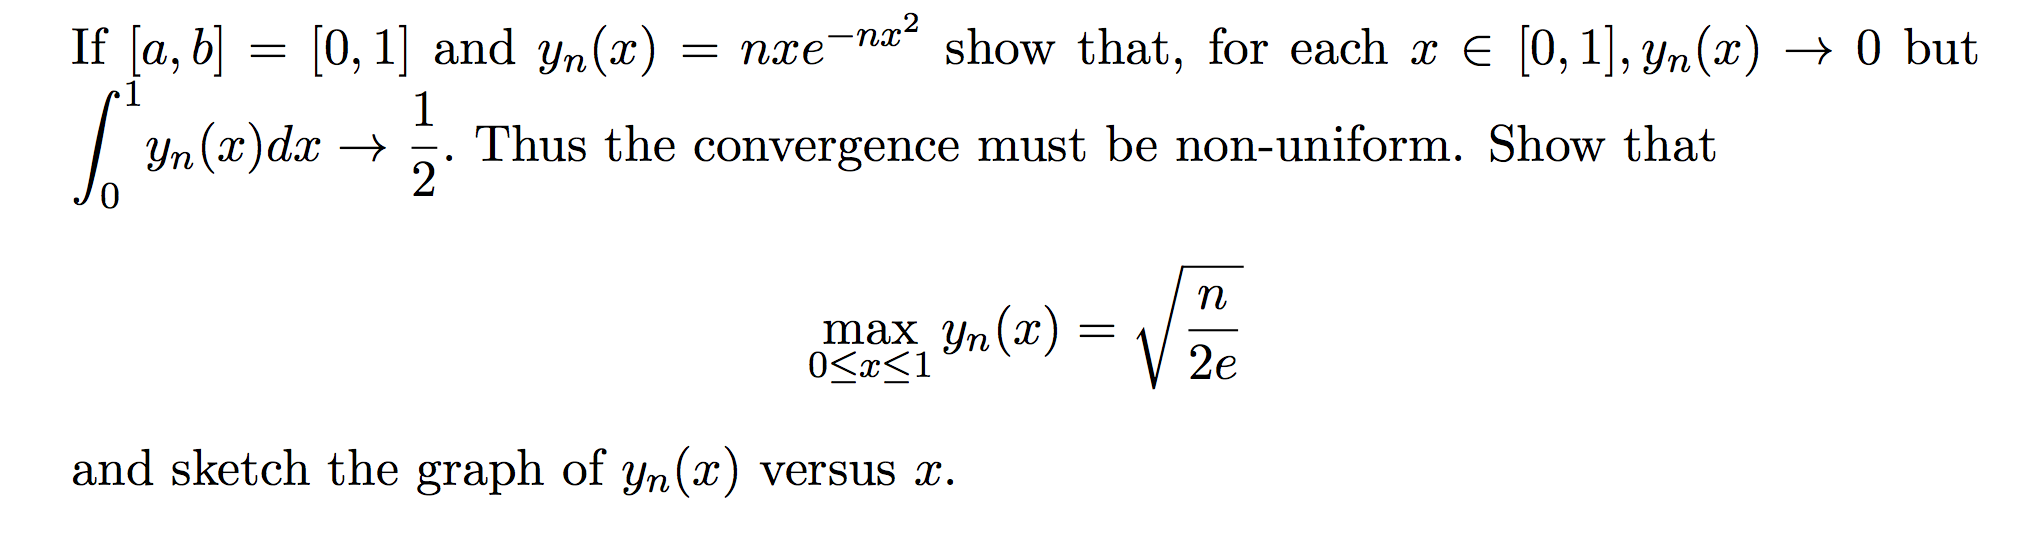
\includegraphics[width=450pt]{img/differential-equations-a1-1-1-b.png}\\
\end{mdframed}

To show that $y_n(x) := \frac{nx}{e^{nx^2}} \to 0$ for all $x \in [0,1]$, first
note that it is true for $x = 0$ since $y_n(0) = 0$ for all $n \in \N$. So we
have to show it is true for $x \in (0, 1]$.

Fix $x \in (0, 1]$ and define $f(\alpha) = \frac{\alpha x}{e^{\alpha x²}}$
for $\alpha \in \R$.  $\lim_{\alpha \to \infty} f(\alpha)$ is an
indeterminate form $\frac{\infty}{\infty}$ and we can use l'H\^{o}pital's
rule, differentiating with respect to $\alpha$:
\begin{align*}
  \lim_{\alpha \to \infty} \frac{\alpha x}{e^{\alpha x^2}}
  = \lim_{\alpha \to \infty} \frac{x}{x^2e^{\alpha x^2}} = 0.
\end{align*}

Since $f(\alpha) = y_n$ at integer values of $\alpha$ it follows that
$\lim_{n\to\infty}y_n(x) = 0$ for all $x \in (0, 1]$. \qed

For the limit of the definite integral we have
\begin{align*}
  \int_0^1 nxe^{-nx^2} \dx
  = \Big[-\frac{1}{2}e^{-nx^2}\Big]_0^1 = \frac{1}{2}(1 - e^{-n}),
\end{align*}
and so $\lim_{n \to \infty} \int_0^1 y_n(x) \dx = \frac{1}{2}$. \qed

To find the maximum value attained by $y_n(x)$ for $x \in [0,1]$, note that the
derivative is
\begin{align*}
  \frac{\d y_n(x)}{\dx} = nx(-2nx)e^{-nx^2} + ne^{-nx^2} = ne^{-nx^2}(1 - 2nx^2),
\end{align*}
and therefore that the only solution to $\frac{\d y_n(x)}{\dx} = 0$ for
$x \in [0,1]$ is $x = \frac{1}{\sqrt{2n}}$.

The second derivative is
\begin{align*}
  % \frac{\d}{\dx} ne^{-nx^2}(1 - 2nx^2) =
  ne^{-nx^2}(-4nx) -2n^2xe^{-nx^2}(1 - 2nx^2)
  = 2n^2xe^{-nx^2}\(2nx^2 - 3\).
\end{align*}
This is negative at the critical point $x = \frac{1}{\sqrt{2n}}$ showing that
it is a maximum. Therefore
\begin{align*}
  \max_{x \in [0,1]} y_n(x)
  = n\frac{1}{\sqrt{2n}}e^{-n(\frac{1}{\sqrt{2n}})^2}
  = \sqrt{\frac{n}{2e}}. \qed
\end{align*}

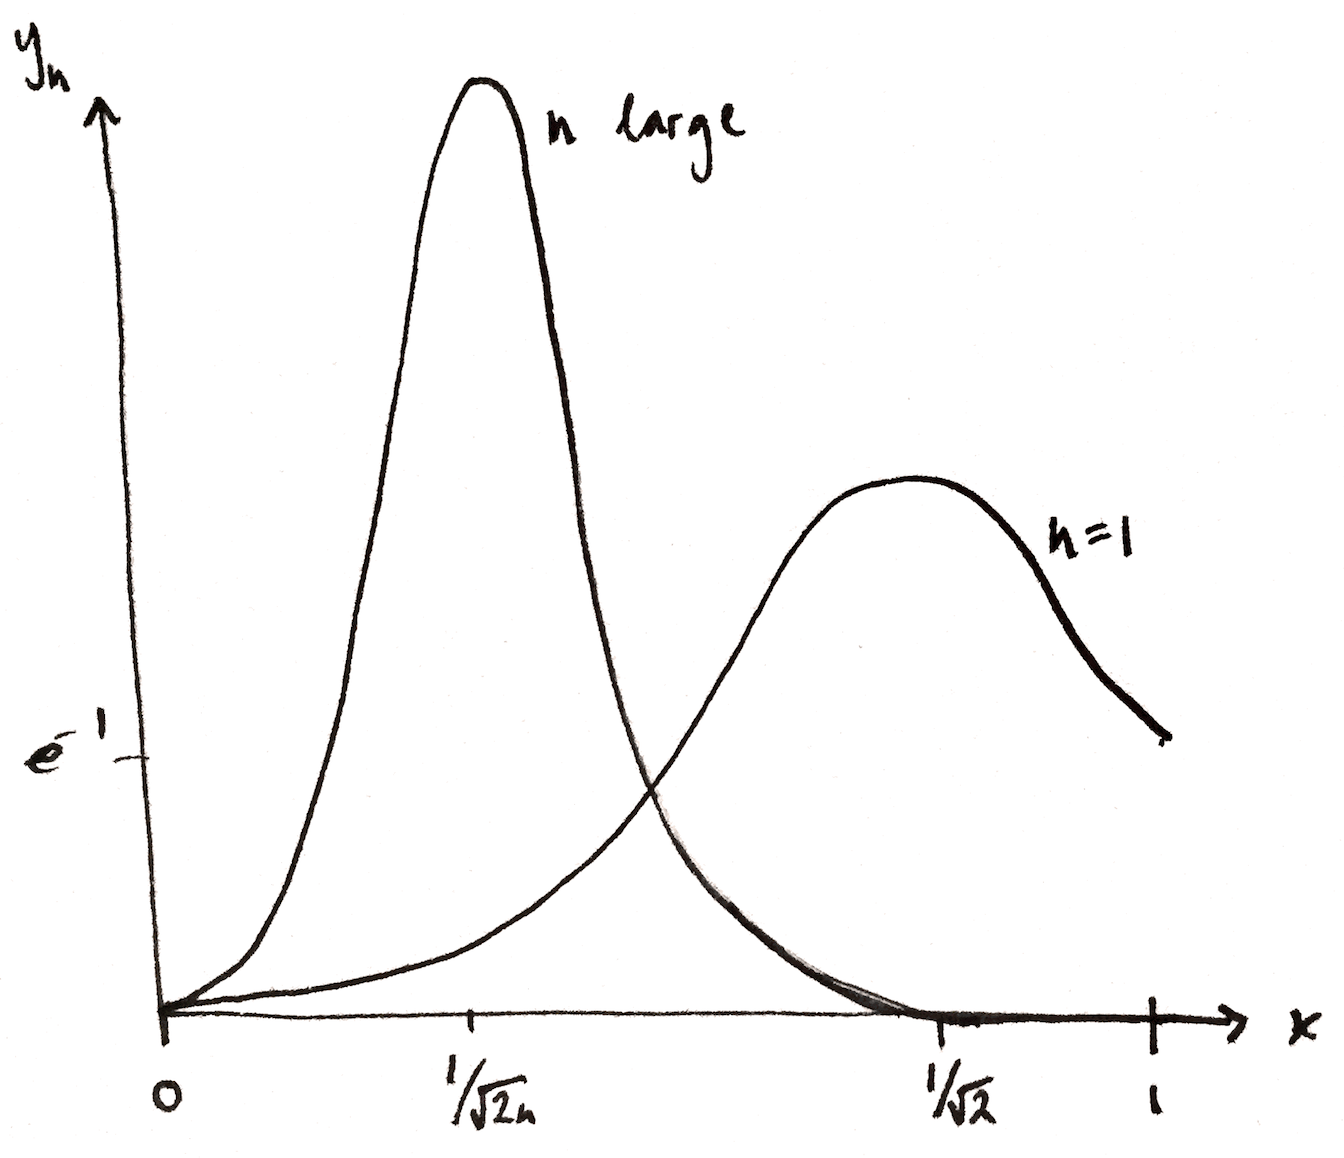
\includegraphics[width=200pt]{img/differential-equations-a1-1-2-diagram.png}\\

\blue{(Approximate time for reading and producing answer: 3 hrs)}

\newpage
\subsection*{} % 2
\begin{mdframed}
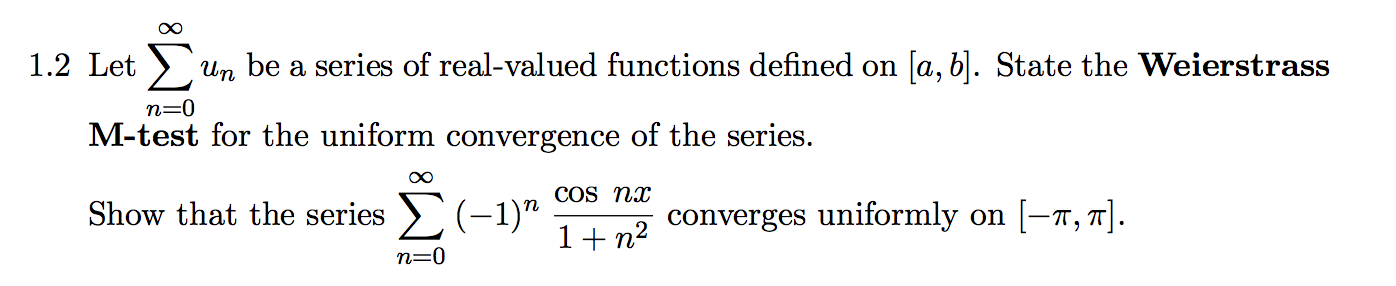
\includegraphics[width=400pt]{img/differential-equations-a1-1-2.png}\\
\end{mdframed}

\subsubsection*{Weierstrass M-test}
Suppose
\begin{enumerate}
\item there exists a sequence $(M_n)_{n\geq 0}$ such that $|u_n(x)| \leq M_n$
  for all $n \geq 0$ and for all $x \in [a,b]$, and
\item the series $\sum_{n=0}^\infty M_n$ converges.
\end{enumerate}

Then the series of functions $\sum_{n=0}^\infty u_n$ converges uniformly on $[a,b]$.

~\\
Define $u_n(x) = (-1)^n ~ \frac{\cos nx}{1 + n^2}$.

Let $M_n = \frac{1}{1 + n^2}$ and note that $|u_n| \leq M_n$ for all
$x \in [-\pi,\pi]$.

Note that the integral
$\int_1^\infty \frac{1}{x^2} \dx = [-\frac{1}{x}]_1^\infty = 1$ converges,
therefore the series $\sum_{n=1}^\infty \frac{1}{n^2}$ converges by the
integral test for convergent series.

Now $M_n < \frac{1}{n^2}$ for $n > 0$, so the series $\sum_{n=1}^\infty M_n$
converges. Therefore the series $\sum_{n=0}^\infty M_n$ also converges, since
its tail converges.

Therefore the series $\sum_{n=0}^\infty u_n$ converges uniformly on
$[-\pi,\pi]$.

\newpage
\subsection*{}  % 3
\begin{mdframed}
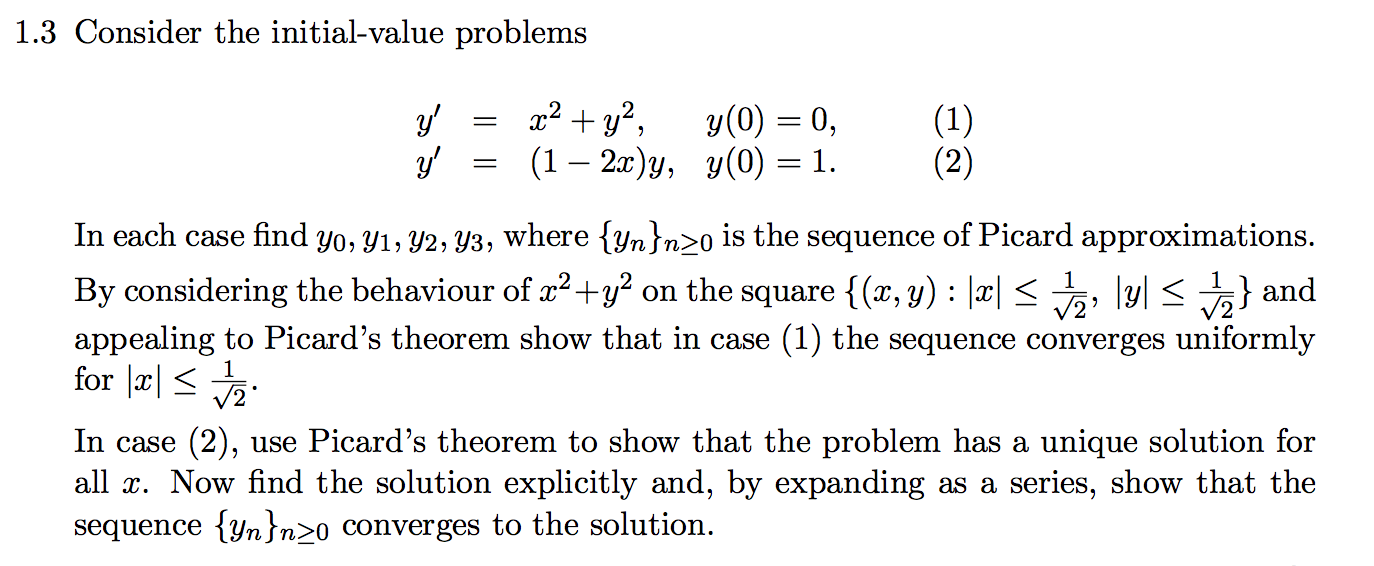
\includegraphics[width=400pt]{img/differential-equations-a1-1-3.png}\\
\end{mdframed}

Consider an ODE $y' = f\Big(x, y(x)\Big)$ with initial condition $y(a) = b$.

The sequence of Picard approximations are defined by
\begin{align*}
  y_0(x)    &= b\\
  y_{n+1}(x) &= b + \int_a^x f\Big(t, y_n(t)\Big) \dt.
\end{align*}

\subsubsection*{(1)}
\begin{align*}
  y_0(x) &= 0\\
  y_1(x) &= 0 + \int_0^x t^2 + 0^2 \dt\\
         &= \frac{x^3}{3}\\
  y_2(x) &= 0 + \int_0^x t^2 + \(\frac{t^3}{3}\)^2 \dt
          = 0 + \int_0^x t^2 + \frac{t^6}{9}\\
         &= \frac{x^3}{3} + \frac{x^7}{63}\\
  y_3(x) &= 0 + \int_0^x t^2 + \(\frac{t^3}{3} + \frac{t^7}{63}\)^2 \dt
          = 0 + \int_0^x t^2 + \frac{t^6}{9} + \frac{2t^{10}}{189} + \frac{t^{14}}{3969} \dt\\
         & = \frac{x^3}{3} + \frac{x^7}{63} + \frac{2x^{11}}{2079} + \frac{x^{15}}{59535}
\end{align*}

We need to show that this situation satisfies the requirements of Picard's
theorem.

Define $v(x, y) = x^2 + y^2$ and let $h = \frac{1}{\sqrt{2}}$ be half the width
of the square, which is centered at $(0, 0)$.

\begin{enumerate}
\item \textbf{$|v|$ must be bounded by some $M>0$ in the rectangle, with $Mh \leq h$}\\
  True. The maximum value attained by $|v|$ in the rectangle is $M = 1$.
\item \textbf{$v$ must be Lipschitz continuous in $y$}\\
  True. The maximum value of $|\partiald{v}{y}|$ on the rectangle is
  $2\cdot\frac{1}{\sqrt{2}} = \sqrt{2}$. Let $(x, y_0)$ and $(x, y_1)$ be two
  points lying on a line parallel to the $y$ axis in the rectangle. By the Mean
  Value Theorem, the partial derivative at some point in this line is equal to
  the slope of the line joining $v(x, y_0)$ and $v(x, y_1)$. Therefore the
  slope of this line cannot exceed $\sqrt{2}$. I.e.
  $|v(x, y_1) - v(x, y_0)| \leq \sqrt{2}|y_1 - y_0|$; $v$ is Lipschitz
  continuous in the $y$ direction within the rectangle.
\end{enumerate}

Therefore the sequence of functions given by the Picard iterates
$y_0, y_1, \ldots$ converge uniformly to a solution of the ODE on
$|x| \leq \frac{1}{\sqrt{2}}$.\\\\

\newpage
\begin{mdframed}
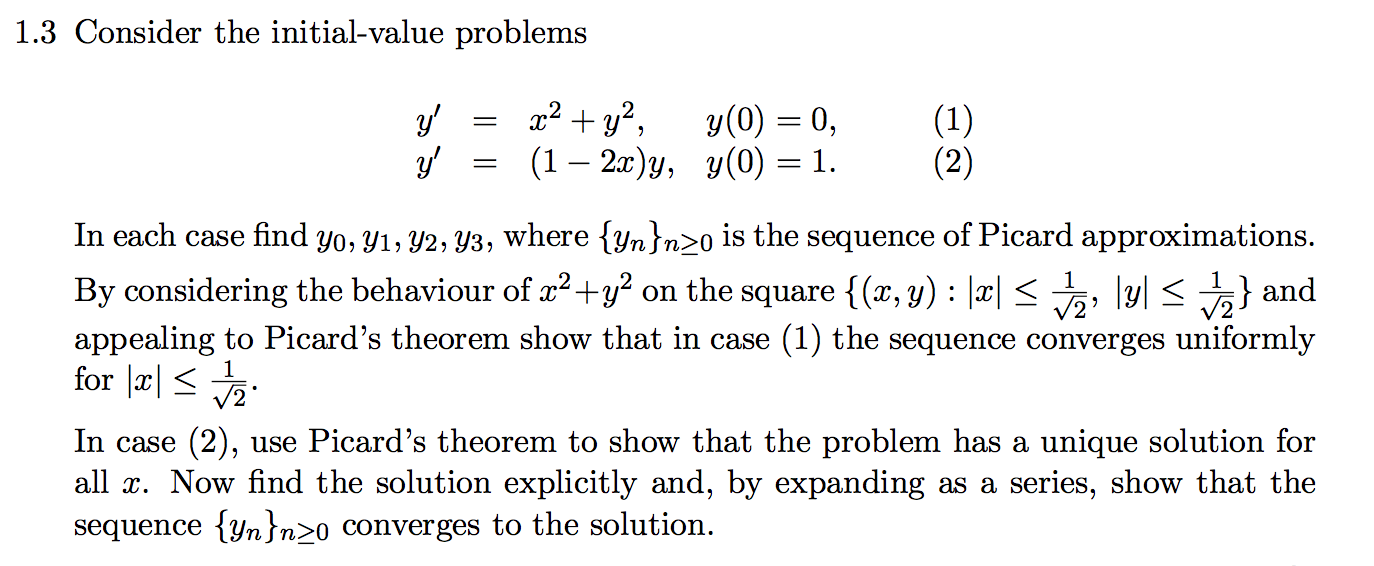
\includegraphics[width=400pt]{img/differential-equations-a1-1-3.png}\\
\end{mdframed}
\subsubsection*{(2)}
\subsubsection*{Show that a unique solution exists for all $x$}
The ODE is
\begin{align*}
  y'(x) = (1 - 2x)y.
\end{align*}

Let $v(x, y) = (1 - 2x)y$ and define an arbitrary rectangle
$\{(x, y) ~:~ |x| \leq h, |y| \leq k\}$.

\begin{enumerate}
\item \textbf{$|v|$ must be bounded by some $M>0$ in the rectangle, with $Mh \leq k$}\\
  \red{False. The maximum value attained by $|v|$ in the rectangle is
    $M=(1+2h)k$. Therefore $Mh = h(1 + 2h)k > k$.} But this contradicts the
  question.

\item \textbf{$v$ must be Lipschitz continuous in $y$}\\
  The maximum value of $|\partiald{v}{y}|$ on the rectangle is $1 + 2h$, so $v$
  is Lipschitz continuous in the $y$ direction.
\end{enumerate}


\subsubsection*{Find the solution via Picard's theorem}

Picard iterates are
\begin{align*}
  y_0(x) &= 1\\
  y_1(x) &= 1 + \int_0^x (1 - 2t)\cdot 1 \dt\\
         &= 1 + [t - t^2]_0^x\\
         &= 1 + x - x^2\\
  y_2(x) &= 1 + \int_0^x (1 - 2t)(1 + t - t^2) \dt\\
         &= 1 + \int_0^x 1 + t - t^2 -2t -2t^2 + 2t^3 \dt\\
         &= 1 + \int_0^x 1 - t - 3t^2 + 2t^3 \dt\\
         &= 1 + x - \frac{1}{2}x^2 - x^3 + 8x^4\\
  y_3(x) &= 1 + \int_0^x (1 - 2t)(1 + t - \frac{1}{2}t^2 - t^3 + \frac{1}{2}t^4)\\
         &= 1 + \int_0^x 1 + t - \frac{1}{2}t^2 - t^3 + \frac{1}{2}t^4 - 2t - 2t^2 + t^3 + 2t^4 - t^5\\
         &= 1 + \int_0^x 1 - t - \frac{5}{2}t^2 + \frac{5}{2}t^4 - t^5\\
         &= 1 + x - \frac{1}{2}x^2 - \frac{5}{6}x^3 + \frac{1}{2}x^5 - \frac{1}{6}x^6
\end{align*}

\begin{mdframed}
\textbf{Check solution with sympy}
\begin{minted}{python3}
from sympy import latex, integrate, symbols
t, y, tau = symbols('t y tau')

def picard(f, y_prev, a, b):
    return b + integrate(f.subs([(t, tau), (y, y_prev)]), (tau, a, t))

a, b = 0, 1

y = b
for i in [1, 2, 3]:
    f = (1 - 2*t) * y
    y_next = picard(f, y, a, b)
    print(latex(y_next))
    y = y_next
\end{minted}
\begin{align*}
  - t^{2} + t + 1\\
  \frac{t^{4}}{2} - t^{3} - \frac{t^{2}}{2} + t + 1\\
  - \frac{t^{6}}{6} + \frac{t^{5}}{2} - \frac{5 t^{3}}{6} - \frac{t^{2}}{2} + t + 1\\
\end{align*}
\end{mdframed}

\subsubsection*{Find the solution explicitly}
Find general solution using separation of variables:
\begin{align*}
  \dydx &= (1 - 2x)y\\
  \frac{1}{y}\dydx &= (1 - 2x)\\
  \int \frac{1}{y} \dydx \dx &= \int (1 - 2x)y \dx
\end{align*}
(Note\footnote{We don't use the Leibnitz notation to perform
  ``cancellations''. This is asking for the antiderivative, with respect to
  $x$, of $\frac{1}{y(x)}y'(x)$, the answer to which is $\log(y(x)) + C$.})
\begin{align*}
  \log y  &= x - x^2 + C\\
  y &= Ae^{x(1-x)}
\end{align*}
Use initial values to find particular solution:
\begin{align*}
  1 &= Ae^0 = A\\
  y(x) &= e^{x - x^2}
\end{align*}
The first few derivatives, evaluated at $x=0$, are
\begin{align*}
y^{(1)}(0) &= (1 - 2x)e^{x - x^2}\\
           &= 1\\
y^{(2)}(0) &= (1 - 2x)^2e^{x - x^2} + (-2)e^{x - x^2}\\
          &= (4x^2 - 4x - 1)e^{x - x^2}\\
           &= -1\\
y^{(3)}(0) &= (4x^2 - 4x - 1)(1 - 2x)e^{x - x^2} + (8x - 4)e^{x - x^2}\\
           &= (4x^2 - 4x - 1 - 8x^3 + 8x^2 + 2x + 8x - 4)e^{x - x^2}\\
           &= (-8x^3 +12x^2 + 6x -5)e^{x - x^2}\\
           &= -5
\end{align*}

The Taylor series expansion of the solution around $x=0$ is
\begin{align*}
  y(x) &= e^{x - x^2}\\
       &= \sum_{n=0}^\infty \frac{y^{(n)}(0)}{n!} x^n\\
       &= 1 + x - \frac{x^2}{2} - \frac{5}{6}x^3 + \ldots.
\end{align*}
So the first few terms appear to match the Picard iterates.

\red{TODO: prove that the Picard iterates converge to the Taylor series.}



\subsection*{}  % 4
\begin{mdframed}
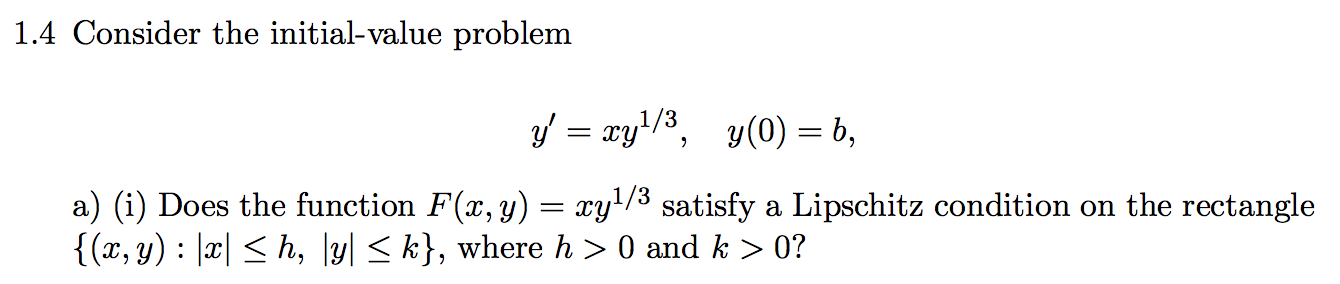
\includegraphics[width=400pt]{img/differential-equations-a1-1-4-a.png}
\end{mdframed}
The partial derivative with respect to $y$ is
$\partiald{F}{y} = \frac{x}{3}y^{-2/3}$.

Note that the rectangle necessarily includes the origin. But
$\partiald{F}{y} \to \infty$ as $y \to 0$. So $F$ does not satisfy a Lipschitz
condition in the $y$ direction.\\

\newpage
\begin{mdframed}
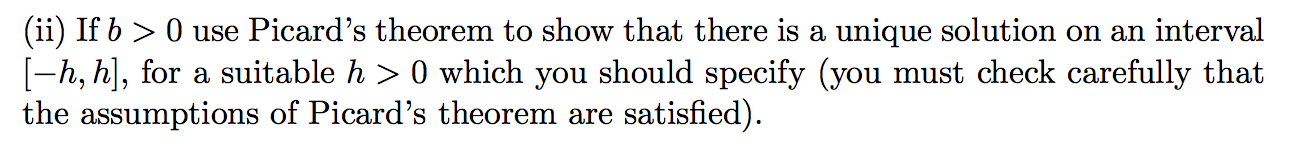
\includegraphics[width=400pt]{img/differential-equations-a1-1-4-b.png}
\end{mdframed}

First note that we can solve this by separation-of-variables:
\begin{align*}
  y' &= xy^{1/3}\\
  \int y^{-1/3} \dy  &= \int x \dx\\
   \frac{3}{2}y^{2/3}  &= \frac{1}{2}x^2 + C\\
    y &= \(\frac{1}{3}x^2 + C\)^{3/2}\\
    y(0) &= C^{3/2} = b\\
    y &= \(\frac{1}{3}x^2 + b^{2/3}\)^{3/2}\\
\end{align*}


\newpage
\begin{mdframed}
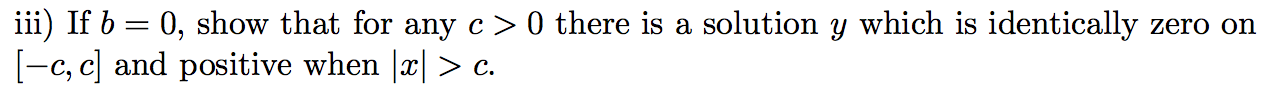
\includegraphics[width=400pt]{img/differential-equations-a1-1-4-c.png}
\end{mdframed}
\begin{mdframed}
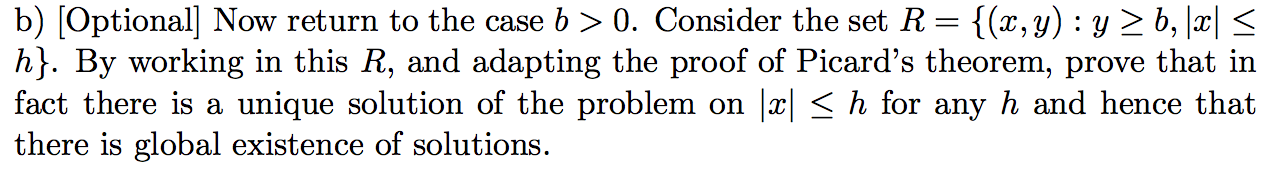
\includegraphics[width=400pt]{img/differential-equations-a1-1-4-d.png}
\end{mdframed}
\end{comment}

\newpage
\subsection*{}  % 5
\begin{mdframed}
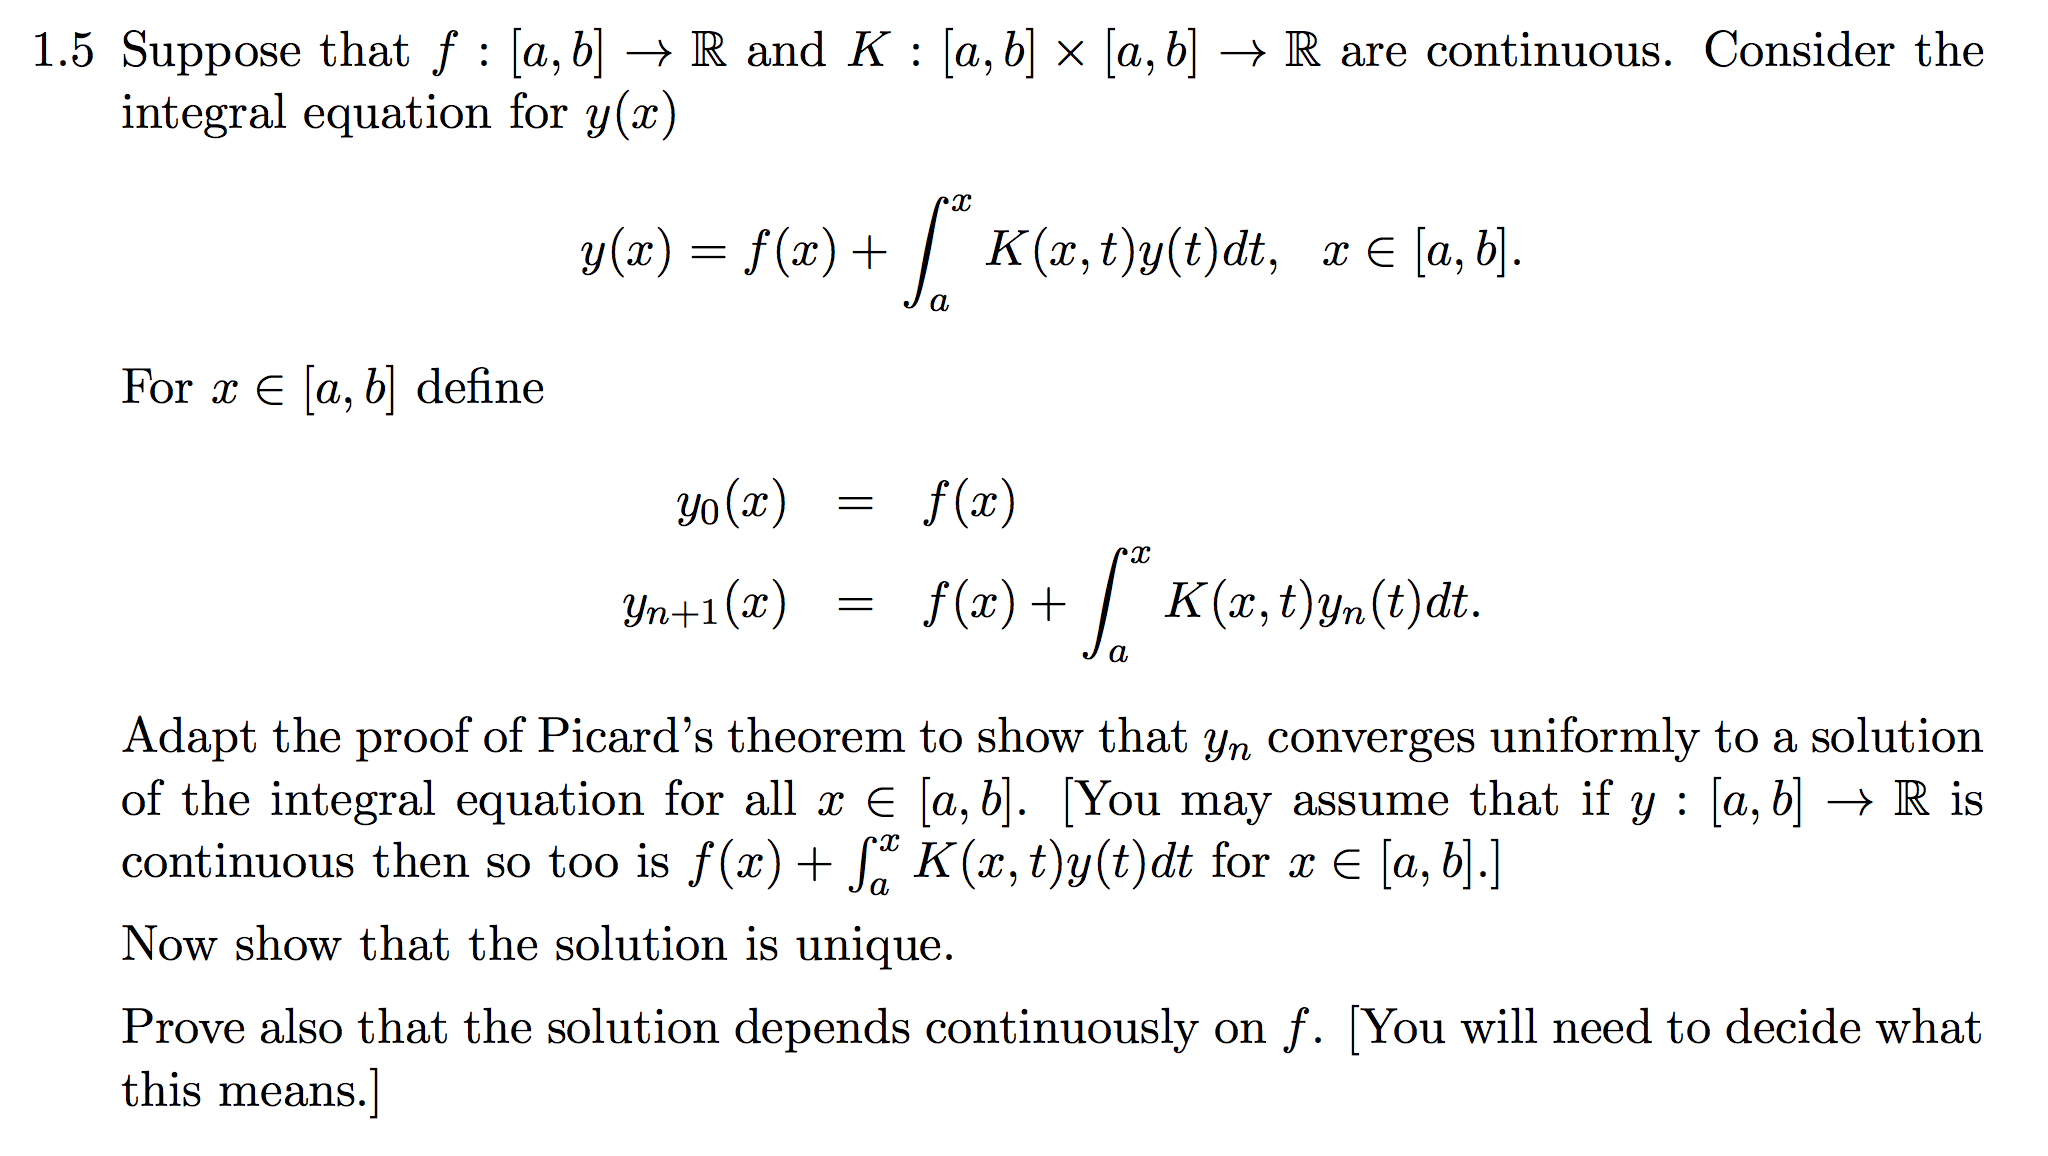
\includegraphics[width=400pt]{img/differential-equations-a1-1-5.png}
\end{mdframed}

We have to show the following:
\begin{enumerate}
\item that the sequence of functions converges uniformly to a limiting function,
\item that the limiting function is a solution, and
\item that the solution is unique, and
\item that the solution ``depends continuously on $f$''.
\end{enumerate}

\subsubsection*{1. Proof that the sequence converges uniformly to a limiting function}

\begin{proof}
Restrict attention to a rectangle with width $2h$ and height $2k$, centered
on $(a, f(a))$.

Note that, since $f$ and $K$ are continuous, there exist bounds $B, C \in \R$
such that $\Big|f(x)\Big| < B$ and $\Big|K(x, x')\Big| \leq C$, for
$x, x' \in [a,b]$.

Define $y_\infty = \limn y_n$.

Define $e_n(x) = y_{n+1}(x) - y_n(x)$.

Note that $y_\infty(x) = \sum_{i=0}^\infty e_n(x) + y_0(x) = \sum_{i=0}^\infty e_n(x) + f(x)$.

Therefore, to show that $(y_n)_{n\geq 0}$ converges uniformly, it suffices to
show that $\sum_{i=0}^\infty e_n(x)$ converges uniformly.

We will use the Weierstrass M-test for this. Therefore, for each $n$ we need to
find a constant bound $W_n$ such that $|y_n(x)| \leq W_n$ for all
$x \in [a,b]$, and we need to show that the sequence $W_n$ converges.

Note that for $n \geq 1$
\begin{align*}
  |e_n(x)| &   = \Bigg|\int_a^x K(x, t) \Big(y_n(x) - y_{n-1}(x)\Big)\dt\Bigg|\\
           &\leq \Bigg|\int_a^x \Big|K(x, t)\Big| \Big|y_n(x) - y_{n-1}(x)\Big|\dt\Bigg|\\
           &\leq \Bigg|\int_a^x \Big|K(x, t)\Big| \Big|e_{n-1}(t)\Big|\dt\Bigg|.
\end{align*}
The first two terms are
\begin{align*}
  |e_0(x)| &=    y_1(x) - f(x)\\
           &=    \int_a^x K(x, t) f(t)\dt\\
           &\leq BC|x - a|\\
  |e_1(x)| &\leq \Bigg|\int_a^x \Big|K(x, t)\Big| \Big|e_0(t)\Big|\dt\Bigg|\\
           &\leq BC\Bigg|\int_a^x \Big|K(x, t)\Big| \Big|t - a\Big| \dt\Bigg|\\
           &\leq BC^2\frac{|x - a|^2}{2}.
\end{align*}
Let $W_n = BC^{n+1}\frac{h^{n+1}}{(n+1)!}$.

It seems that $|e_n(x)| \leq W_n$ for all $n \geq 0$. To prove this, note that
it is true for $n=0$. For induction, suppose that it is true for $n$. Then
\begin{align*}
  |e_{n+1}(x)|& \leq \Bigg|\int_a^x \Big|K(x, t)\Big| \Big|e_{n}(t)\Big|\dt\Bigg|\\
             & \leq \Bigg|\int_a^x \Big|K(x, t)\Big| BC^{n+1}\frac{(t - a)^{n+1}}{(n+1)!^{~~~~}}\dt\Bigg|\\
             & \leq BC^{n+2}\frac{(x - a)^{n+2}}{(n+2)!^{~~~}}\\
             & \leq BC^{n+2}\frac{h^{n+2}}{(n+2)!}\\
             &= W_{n+1},
\end{align*}
as required. Therefore $|e_n| \leq W_n$ holds for all $n \geq 0$. The Ratio
Test shows that the sequence $(W_n)_{n\geq 0}$ converges to zero:
\begin{align*}
  \limn \frac{W_{n+1}}{W_n}
  = \limn \frac{BC^{n+2}\frac{h^{n+2}}{(n+2)!}}
                {BC^{n+1}\frac{h^{n+1}}{(n+1)!}}
  = \limn \frac{Ch}{n+2}
  = 0.
\end{align*}
Therefore the series $\sum_{i=0}^\infty e_n(x)$ converges uniformly by the
Weierstrass M-test, and therefore $(y_n)_{n\geq 0}$ converges uniformly to a
limiting function, which we will denote as $y_\infty$.
\end{proof}

\subsubsection*{2. Proof that the limiting function is a solution}

\begin{proof}
To prove that $y_\infty$ is a solution we need to show that
\begin{align*}
  y_\infty(x) = \limn y_n(x) = f(x) + \int_a^x K(x, t) y_\infty(t) \dt
  ~~~~~~~\text{and}~~~~~~~
  y_\infty(a) = f(x).
\end{align*}
The second requirement, $y_\infty(a) = f(x)$, is clearly true.

The definition of $y_n$ is
\begin{align*}
  y_n(x) = f(x) + \int_a^x K(x, t) y_{n-1}(t) \dt.
\end{align*}
If it were valid to take the limit inside the integral then we would have
\begin{align*}
  y_\infty(x) = \limn y_n(x) = f(x) + \int_a^x K(x, t) y_\infty(t) \dt
\end{align*}
as required. To justify taking the limit inside the integral it's sufficient to
prove that $K(x, t) y_{n}(t)$ converges uniformly to $K(x, t) y_\infty(t)$. But
this simply requires that $y_{n}(t)$ converges uniformly to $y_\infty(t)$,
which has been proved already.
\end{proof}

\subsubsection*{3. Proof that the solution is unique}

\begin{proof}
Suppose that $Y$ is a solution and define $e_n(x) = Y(x) - y_n(x)$. We will
show that $\limn |e_n(x)| = 0$.

Recall that we are working in a rectangle with width $2h$ and height $2k$,
centered on $(a, f(a))$.

We have
\begin{align*}
  |e_0(x)| &=    \Bigg|\int_a^x K(x,t)Y(t) \dt\Bigg|\\
           &\leq \Bigg|\int_a^x \Big|K(x,t)\Big|\Big|Y(t)\Big| \dt\Bigg|\\
           &\leq Ck|x-a|.
\end{align*}

For $n \geq 1$ we have
\begin{align*}
  |e_n(x)| &= \Bigg|\int_a^x K(x,t)\Big(Y(t) - y_{n-1}(t)\Big) \dt\Bigg|\\
           &\leq \Bigg|\int_a^x \Big|K(x,t)\Big|\Big|d_{n-1}(t)\Big|\dt\Bigg|\\
\end{align*}
For induction, suppose that $|e_n(x)| \leq
C^{n+1}k\frac{|t-a|^{n+1}}{(n+1)!}$. This is true for $n=0$. For $n+1$, we have
\begin{align*}
|e_{n+1}(x)| &\leq \Bigg|\int_a^x \Big|K(x,t)\Big|\Big|d_{n}(t)\Big|\dt\Bigg|\\
            &=    \Bigg|\int_a^x \Big|K(x,t)\Big|C^{n+1}k\frac{|t-a|^{n+1}}{(n+1)!}\dt\Bigg|\\
            &=    C^{n+2}k\frac{|t-a|^{n+2}}{(n+2)!}\\
            &\leq C^{n+2}k\frac{h^{n+2}}{(n+2)!},
\end{align*}
which, as shown above, converges to 0 as $n \to \infty$. Therefore
$\limn |e_n(x)| = 0$ and therefore if $Y$ is a solution then $y_\infty = Y$.
\end{proof}

\newpage
\subsubsection*{3. Proof that the solution ``depends continuously on $f$''}

\begin{proof}
  Let $f,g: [a,b] \to \R$ and fix $\epsilon > 0$. Let $y_f(x)$ and $y_g(x)$ be
  solutions to the respective IVPs:
  \begin{align*}
    y_f(x) &= f(x) + \int_a^x K(x, t) y_f(t) \dt\\
    y_g(x) &= g(x) + \int_a^x K(x, t) y_g(t) \dt.
  \end{align*}
We have
\begin{align*}
  \Big|y_f(x) - y_g(x)\Big|
  &\leq \Big|f(x) - g(x)\Big| + \Bigg|\int_a^x K(x, t) y_f(t) - y_g(t) \dt\Bigg|\\
  &\leq \Big|f(x) - g(x)\Big| + C\Bigg|\int_a^x \Big|y_f(t) - y_g(t)\Big| \dt\Bigg|,
\end{align*}
therefore by Gronwall's inequality
\begin{align*}
  \Big|y_f(x) - y_g(x)\Big| &\leq \Big|f(x) - g(x)\Big|e^{C|x-a|}\\
                            &\leq \Big|f(x) - g(x)\Big|e^{Ch}.
\end{align*}
Let $\epsilon > 0$ and let $\delta(\epsilon) = e^{-Ch}\epsilon$. Then the
solution ``depends continuously on $f$'' in the sense that
$\forall ~ x \in [a, b] ~ \forall ~ \epsilon > 0$
\begin{align*}
  \Big|f(x) - g(x)\Big| < \delta(\epsilon) \implies \Big|y_f(x) - y_g(x)\Big| < \epsilon.
\end{align*}
\end{proof}

\hrule

Let $\|g\|$ be the sup norm for a real-valued function $g$ defined on $[a,b]$:
\begin{align*}
  \|g\| := \sup_{x\in [a,b]} \Big|g(x)\Big|.
\end{align*}

We switch notation to make explicit that a solution $y$ depends on the function
$f$. So now $y(f):[a,b]\to\R$ is the solution of the IVP posed with function
$f$. I.e., $y(f)$ satisfies
\begin{align*}
  y(f)(x) = f(x) + \int_a^x K(x, t) ~ y(f)(t) \dt.
\end{align*}

\begin{definition*}
  The solution $y_\infty$ depends continuously on $f$ if for every
  $\epsilon > 0$ there exists $\delta > 0$ such that if $\|f - g\| < \delta$
  then $\|y(f) - y(g)\| < \epsilon$.
\end{definition*}

\begin{claim*}
  $y_\infty$ depends continuously on $f$.
\end{claim*}


\begin{proof}
Let $f,g:[a,b]\to\R$ and fix $\epsilon > 0$.

We have
\begin{align*}
  \Big(y_\infty(f) - y_\infty(g)\Big)(x) =
  \(f - g\)(x) +
  \int_a^x K(x, t) \Big(y_\infty(f) - y_\infty(g)\Big)(t) \dt.
\end{align*}
Therefore
\begin{align*}
  \Big\|y_\infty(f) - y_\infty(g)\Big\| \leq
  \Big\|f - g\Big\| +
  \Bigg\|\int_a^x K(x, t) \Big(y_\infty(f) - y_\infty(g)\Big)(t) \dt\Bigg\|.
\end{align*}
Suppose $\|y_\infty(f) - y_\infty(g)\| \leq \epsilon$. Then
\begin{align*}
  0
  \leq \Big\|f - g\Big\| + (x - a)C\epsilon - \epsilon
     =  \Big\|f - g\Big\| + \epsilon\Big((x - a)C - 1\Big)
\end{align*}




\end{proof}

\end{document}
